\section{Meta Patterns}

\subsection{Reflections (POSA1)}

Lösen übliche Frameworker's Probleme

\begin{itemize}
    \item Teile eines Software Systems austauschen ist schwer
    \item bis jetzt unbekannte Software Komponenten sollen nicht integriert werden
    \item bietet \textcolor{blue}{Flexibility}, \textcolor{blue}{Adaptability} und \textcolor{blue}{Generality}
    \item Bieten die Einrichtung für Konzepte wie
    \begin{itemize}
        \item Dependency Injection
        \item Convention over Configuration
        \item Object-Relation Mapper
        \item Serialization / Deserialization
        \item Plugin Architectures
    \end{itemize}
    \item Most frameworks use Reflection to locate implementations of extension points and hooks
\end{itemize}
\vspace{10pt}
\textbf{Usage}
\begin{itemize}
    \item Classes
    \item Object Attributes
    \item Methods
    \item Class Relationships
\end{itemize}

\subsubsection{Aspects}

\textbf{Introspection}

Die Möglichkeit für ein Programm den eigenen Zustand zu überwachen und somit auch ''Reason about'' (z.B. Abfrage, welche Felder eine Klasse hat, \textcolor{blue}{Query object properties}) \\

\textbf{Intercession}

Die Möglichkeit das ein Programm sein eigener Ausführungs-Zustand modifizieren kann. z.B. Können zur Laufzeit die Objekt-Properties oder andere Attribute modizifiert werden \textcolor{blue}{add another attribute} \textcolor{blue}{exchange code}

\subsubsection{Meta vs. Base Level}

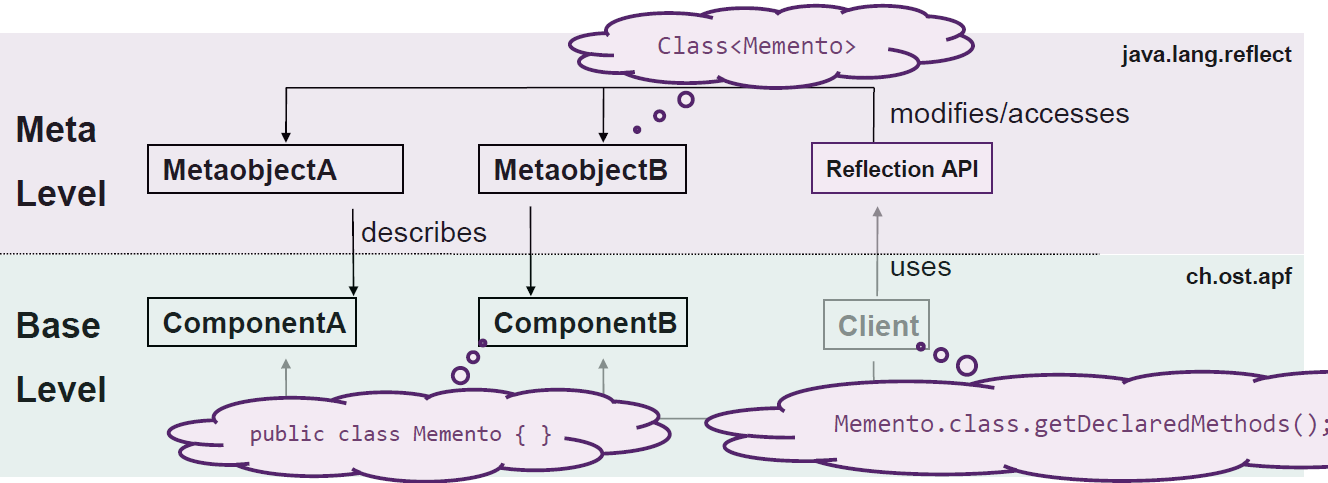
\includegraphics[width=\linewidth]{meta_base_level.png} \\

\textbf{Meta level}
\begin{itemize}
    \item Bietet eine Selbst-Repräsentation
    \item Gibt der Software Wissen über ihre eigene Struktur
    \item Besteht aus Meta-Objekten
    \item Interface für das Manipulieren von Meta-Objekten wird \textcolor{blue}{MOP} genannt
\end{itemize}
\vspace{10pt}
\textbf{Base level}
\begin{itemize}
    \item Definiert die Applikations-Logik
    \item dessen Implementierung kann Meta-Objekte verwenden
\end{itemize}

\subsubsection{Consequences}
\textbf{Benefits}
\begin{itemize}
    \item Ein Software System anpassen ist einfach
    \item Unterstützung für viele Arten von Änderungen
\end{itemize}
\vspace{10pt}

\columnbreak

\textbf{Liabilities}
\begin{itemize}
    \item Produziert nicht-transparente ''black magic'' APIs
    \item Binding zur Laufzeit
    \begin{itemize}
        \item Limitierte Type Safety
        \item Weniger Effizient, keine Compiler-Optimierung
    \end{itemize}
\end{itemize}
\vspace{10pt}
\textbf{Dangers}

\begin{itemize}
    \item Mehr indirection kostet Effizient
    \item Zuviel Arbeit zu konfigurieren und instanzieren des Systems
    \item Resultiert oft in obscure APIs
    \item Overengineered Solutions
    \item Security Mechanismen kommen in den Weg oder werden untergraben
\end{itemize}

\subsection{Type Object (Strategy Pattern)}

Wir wollen übliches Verhalten und Daten an einem Ort haben

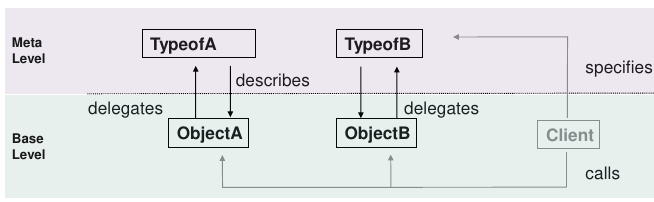
\includegraphics[width=\linewidth]{type-object.png}

\subsubsection{Problem}
\begin{itemize}
    \item We want to keep common behaviour and data in only one place
    \item DRY implementation of domain
    \item How can you categorize objects, eventually dynamically?
\end{itemize}

\subsubsection{Solution}
Kategorisiere Objekte nach einem anderen Objekt anstelle von einer Klasse. Somit kann ein Objekt die Klasse zur Laufzeit ändern

\begin{itemize}
    \item Create a category (type) object which describes multiple objects
    \item Objects forward the calls to the underlying type
\end{itemize}
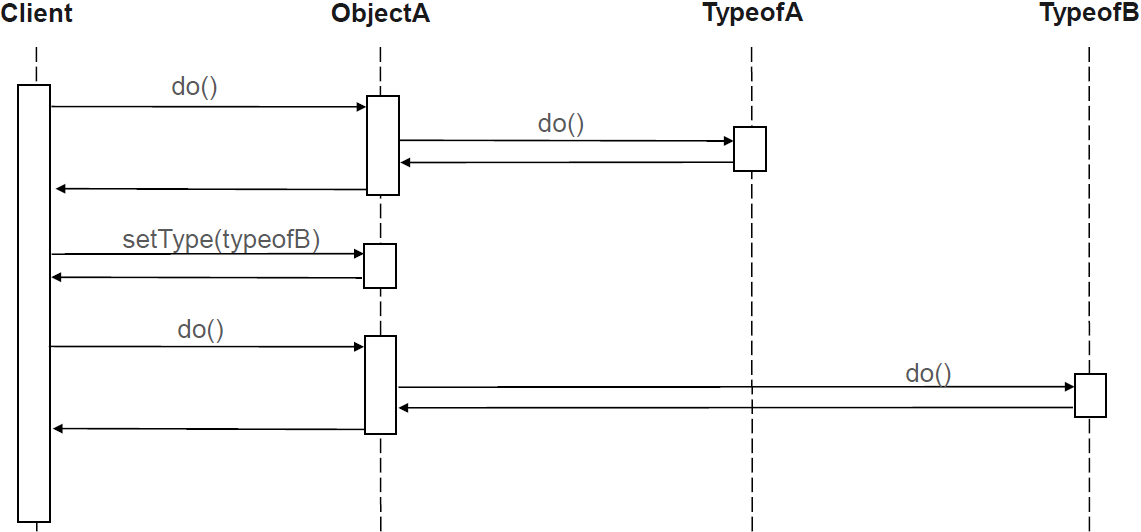
\includegraphics[width=\linewidth]{type_object.png}
\subsubsection{Consequences}
\textbf{Benefits}
\begin{itemize}
    \item Kategorien können einfach hinzugefügt werden
    \item Verhindert eine Explosion von Sub-Klassen
    \item Erlaubt mehrere Meta-Levels
\end{itemize}
\vspace{10pt}
\textbf{Liabilities}
\begin{itemize}
    \item Verwirrendes Mess von Klassen und Klassen Mutationen wegen der Separierung
    \item Weniger Effizienz wegen Indirection
    \item Änderungen von Datenbank Schemas kann tricky sein
\end{itemize}


\subsection{Property List}

Attribute sollen nach der Compilation anbaubar und abbaubar sein. Objekte teilen Attribute / Parameters über die ganze Klassen Hierarchie.

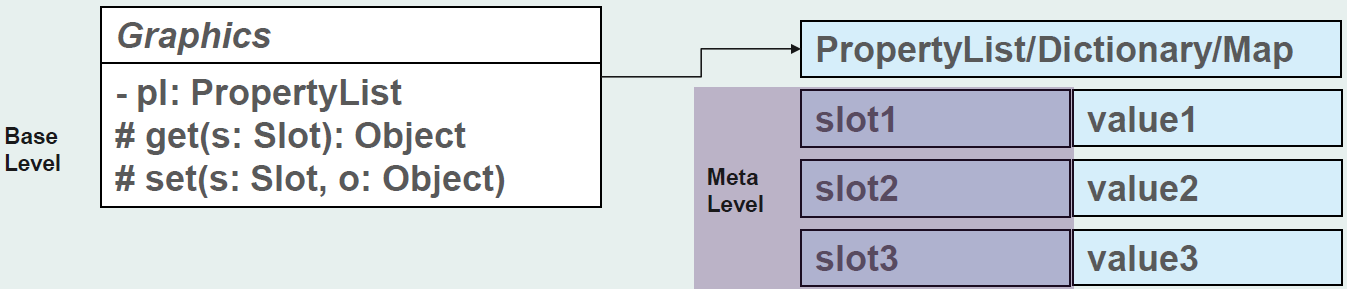
\includegraphics[width=\linewidth]{property_list.png}

\subsubsection{Problem}
\begin{itemize}
    \item Attributes should be attachable / detachable after compilation
    \item Objects share attributes / parameters across the class hierarchy
    \item How do you define properties in a flexible way so they can be attached and detached at runtime?
\end{itemize}

\subsubsection{Solution}
Liefert Objekte mit einer ''Property List''. Diese Liste erlaubt die Verbindung von Namen mit anderen Werten oder Objekten

\begin{itemize}
    \item Property list maps attribute names to values
    \item each name defines a slot
    \item Same slot can be used for attributes with identical semantics
    \item Objects can be triggred to list all slot names and values
\end{itemize}

\subsubsection{Consequences}
\textbf{Benefits}
\begin{itemize}
    \item Black-box Erweiterbarkeit von Attributen, Attribute können dynamisch hinzugefügt werden
    \item Objekt-Erweiterung während Identität gleich bleibt
    \item Gleiche Attribute können für Attribute mit identischer Semantik über die ganze Hierarchie verwendet werden
    \item Flexible Parameters für generische Methoden Interfaces
    \item Easy attribute iteration
\end{itemize}
\vspace{10pt}
\textbf{Liabilities}
\begin{itemize}
    \item Unterschiedliche Wege um auf reguläre und dynamische Attribute zugreifen zu können
    \item Typ-Sicherheit wird dem Programmierer überlassen
    \item Naming wird vom Compiler nicht gecheckt (color vs. colour)
    \item Semantik von Attributen nicht von dem Klassen Code gegeben
    \item Run-Time overhead kann substanziell sein
    \item Memory Management
\end{itemize}

\textcolor{blue}{Bridge Method} kann verwendet werden um type-safety zu mitigieren

\begin{itemize}
    \item Ein typed Schema erlaubt das erzwingen von Property-Namen und Typen
    \item In C\# werden dafür Extension-Methoden verwendet
\end{itemize}

\vfill\null
\columnbreak

\subsection{Anything (Super-Klasse für Typen)}

Wir brauchen eine Map um änhliche Daten zur Property List zu halten. Strukturierte Daten beinhaltet auch Sequenzen von Daten. Daten sollen rekursiv strukuriert sein

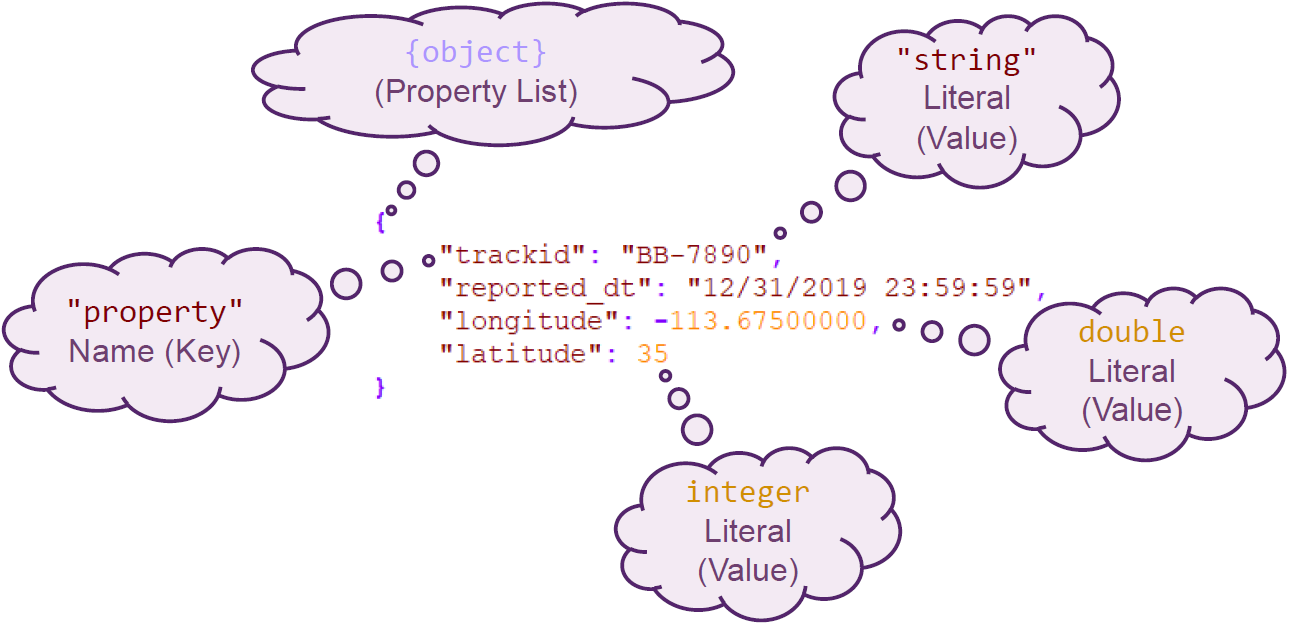
\includegraphics[width=\linewidth]{anything.png}

\subsubsection{Problem}
\begin{itemize}
    \item We need to keep a map of data similar to the Property List
    \item Structured data also includes sequences of data
    \item Data should be structured recursively
    \item How do you provide a generic configuration or communication data structure that is easily extensible?
\end{itemize}

\subsubsection{Solution}
Erstelle eine Abstraktion für strukturiere Werte, welche selbst-beschreibend ist

\begin{itemize}
    \item Implement a representation of simple values
    \item Add an implementation for a sequence of values (\& key value access)
    \item Provide a default value
\end{itemize}
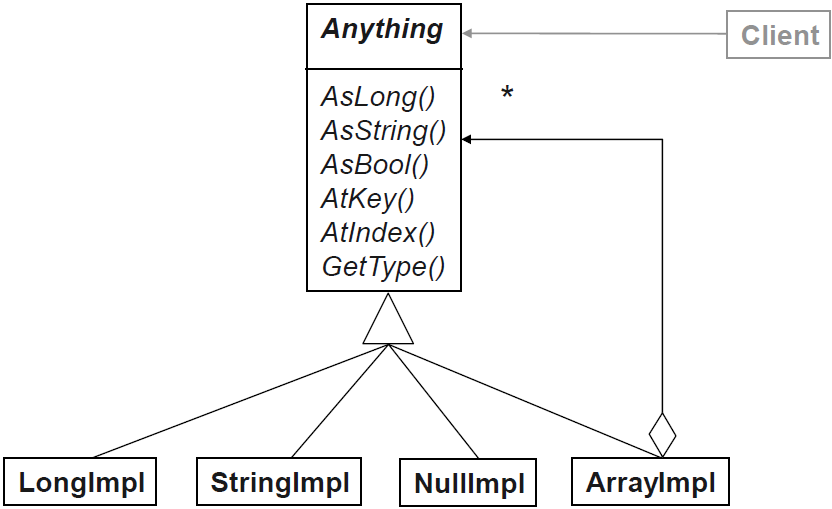
\includegraphics[width=\linewidth]{anything_uml.png}
\subsubsection{Consequences}
\textbf{Benefits}
\begin{itemize}
    \item Lesbares Streaming Format und angemessene Konfigurationsdaten
    \item Universell Anwendbar, flexibler Austausch über Klassen / Objekt Boundaries
    \item Readable streaming format
    \item Appropriate for configuration data
    \item Universally applicable
    \item Flexible interchange across class/object boundaries
\end{itemize}
\vspace{10pt}
\textbf{Liabilities}
\begin{itemize}
    \item Weniger Typ-Sicherheit
    \item Absicht von Parameter Elementen nicht immer obvious
    \item Overhead für Value-Lookup und Member Access
    \item Kein echtes Objekt, nur Daten
\end{itemize}

\subsection{Discussion}
\textbf{On which GoF pattern is Type Object based?}

Strategy Pattern; every type represents an own strategy for item objects \\

\textbf{Have you already encountered a similar intent of a GoF pattern?}

Yes, it’s similar to the State pattern, which ''seems to change its class'' at runtime. \\

\textbf{Which GoF Pattern does Anything (and variation) implement?}
\begin{itemize}
    \item Transparent Composite Pattern
    \item Null Object
\end{itemize}

